\chapter{Visualization}
\section{User Information}
\begin{figure}[h!]
	\centering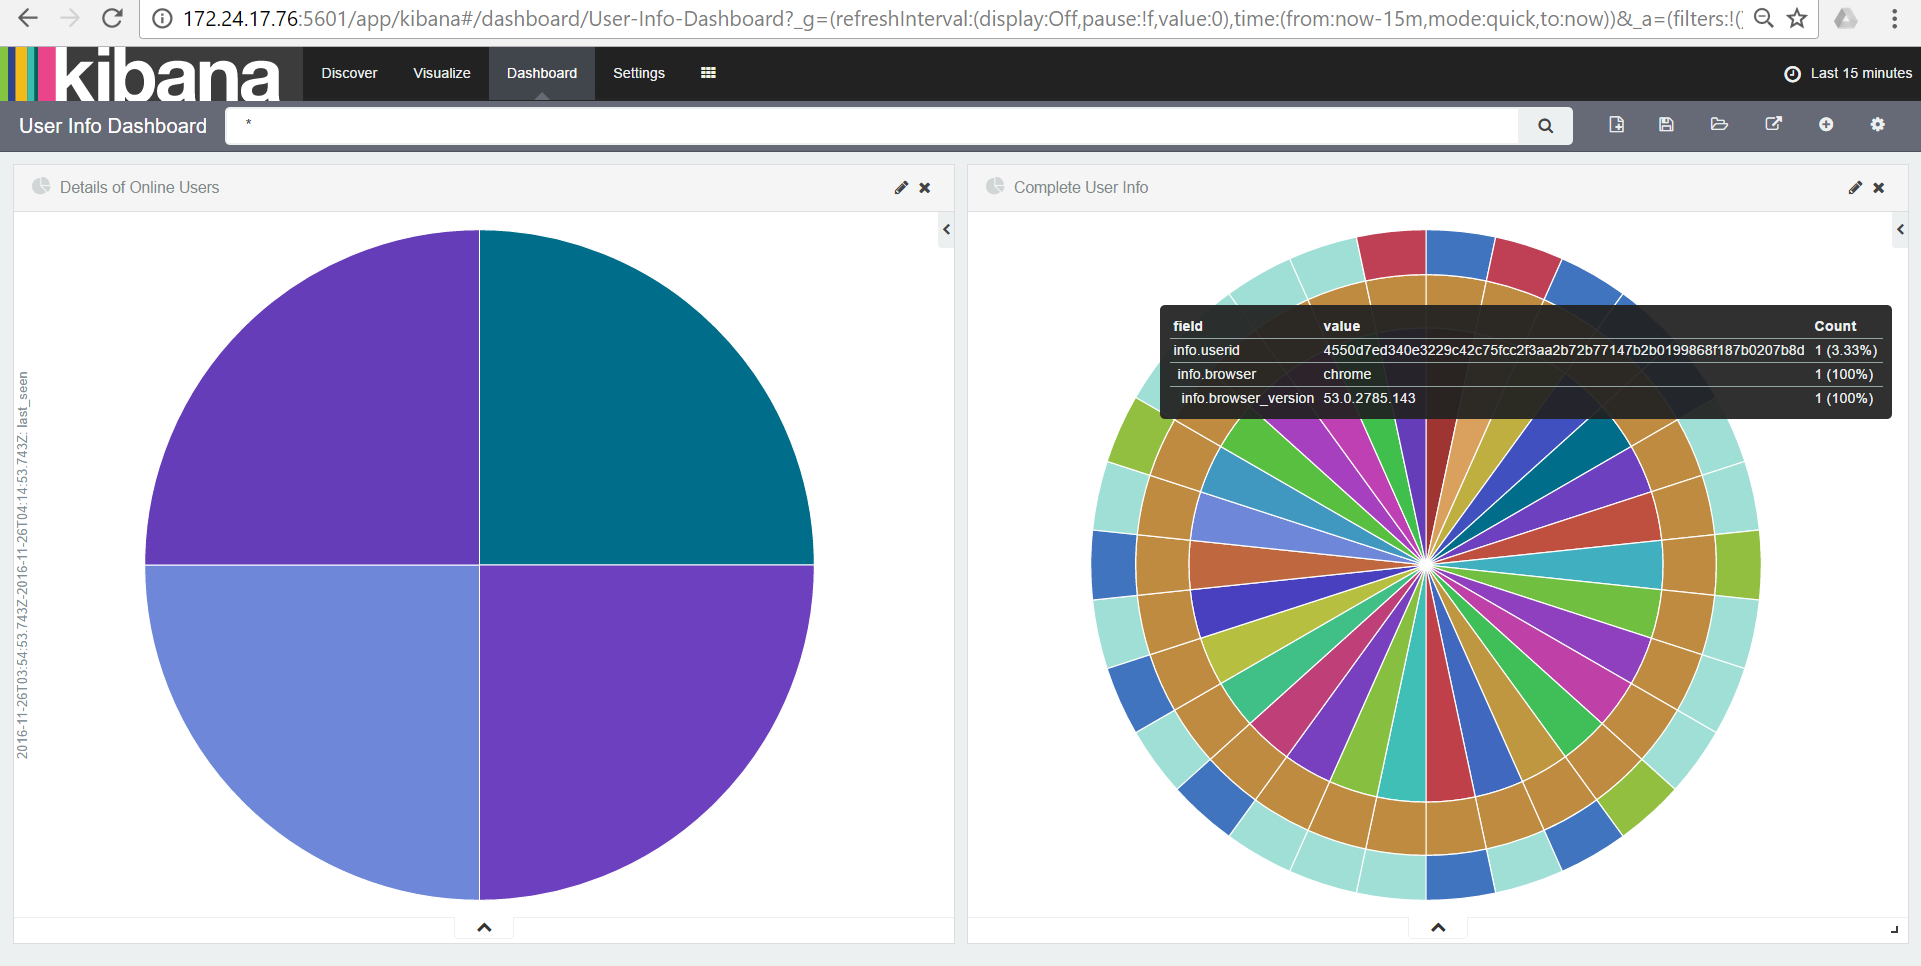
\includegraphics[width=\textwidth,height=\textheight,keepaspectratio]{dashboard.png}
	\caption{Dashboard}
	\label{fig:3}
\end{figure}

\justify Kibana provides us with Dash Boarding capabilities, one example of which can be seen above. The above graph shows the current online users and the relevant info associated with them. While the right picture shows the cookies collected for each user and the urls the cookies are associated with. The visualization can also be done in a simpler tabular form with the correct filters configured.

\begin{figure}[h!]
	\centering\includegraphics[width=\textwidth,height=\textheight,keepaspectratio]{Dashboard.PNG}
	\caption{An example of a dashboard created with filters on Kibana to show User Info.}
	\label{fig:4}
\end{figure}

\chapter{Snapshots}
\begin{figure}[h!]
	\centering\includegraphics[width=\textwidth,height=\textheight,keepaspectratio]{DOM.PNG}
	\caption{A snapshot of a DOM Object Insertion.}
	\label{fig:5}
\end{figure}

\begin{figure}[h!]
	\centering\includegraphics[width=\textwidth,height=\textheight,keepaspectratio]{Phishing.PNG}
	\caption{Snapshot of a phishing attempt.}
	\label{fig:6}
\end{figure}